\documentclass[tikz,border=12pt]{standalone}
\usepackage[utf8]{inputenc}
\usepackage[T1]{fontenc}
\usepackage{lmodern}
\usetikzlibrary{arrows.meta,positioning,shapes.geometric}

\definecolor{geoyellow}{RGB}{246,216,74}
\definecolor{geoborder}{RGB}{161,118,0}
\definecolor{terrred}{RGB}{236,112,108}
\definecolor{terrborder}{RGB}{153,45,42}
\definecolor{paisred}{RGB}{204,24,24}
\definecolor{paisborder}{RGB}{120,10,10}
\definecolor{slate}{RGB}{51,65,85}
\definecolor{navy}{RGB}{24,58,92}

\begin{document}
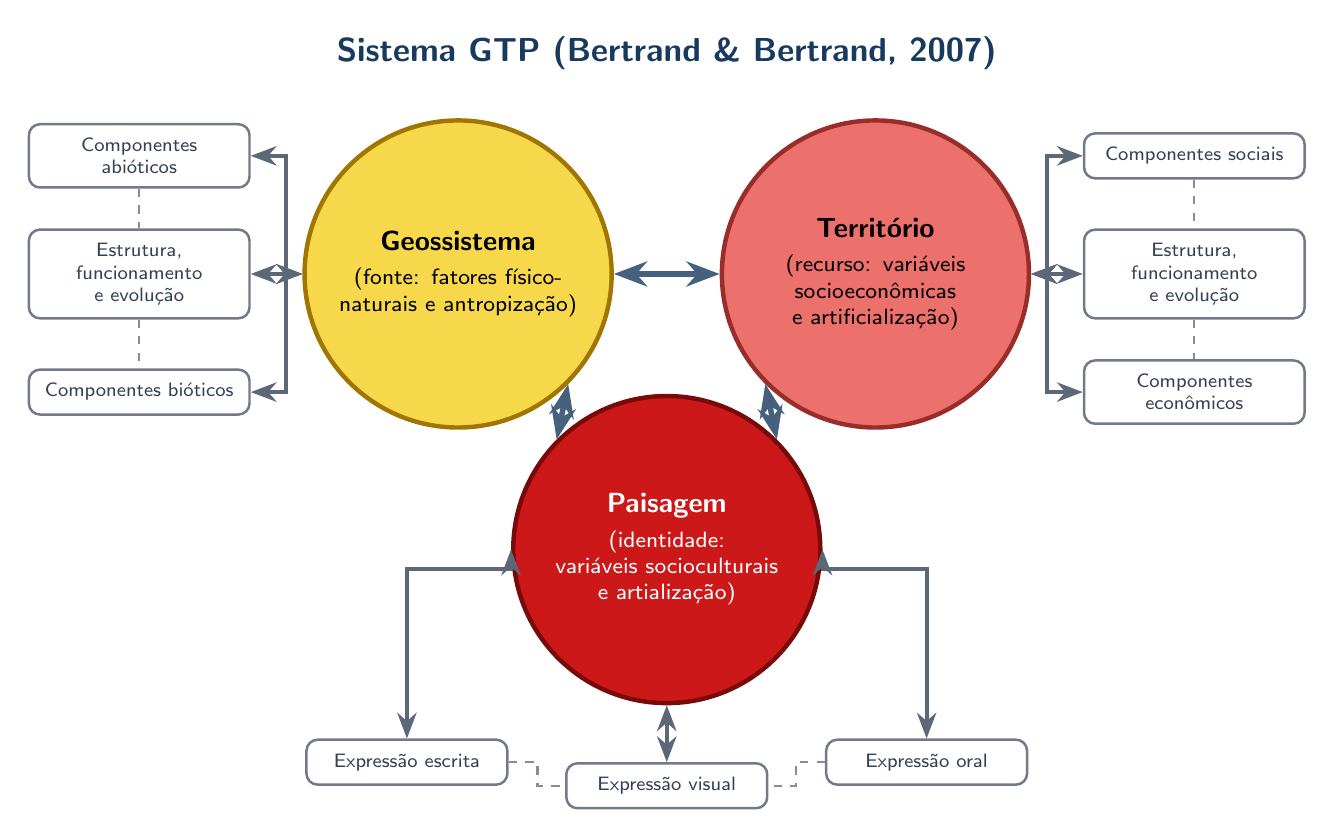
\begin{tikzpicture}[
  font=\sffamily,
  >=Stealth,
  gtpcircle/.style={
    circle, line width=1.6pt,
    minimum size=3.9cm, text width=3.2cm, align=center,
    font=\sffamily\footnotesize
  },
  sidebox/.style={
    rectangle, rounded corners=4pt, draw=slate!70, line width=0.9pt,
    fill=white, text width=2.45cm, align=center, inner sep=5pt,
    font=\sffamily\scriptsize, text=slate
  },
  botbox/.style={
    rectangle, rounded corners=4pt, draw=slate!70, line width=0.9pt,
    fill=white, text width=2.2cm, align=center, inner sep=5pt,
    font=\sffamily\scriptsize, text=slate
  },
  conn/.style={<->, line width=1.4pt, color=slate!80},
  dashlink/.style={dashed, line width=0.8pt, color=slate!60},
  triarrow/.style={<->, line width=2.0pt, color=navy!80}
]

% Título discreto
\node[font=\sffamily\bfseries\large, text=navy] at (0, 4.35) {Sistema GTP (Bertrand \& Bertrand, 2007)};

% Três círculos centrais
\node[gtpcircle, draw=geoborder, fill=geoyellow, text=black] (G) at (-2.65, 1.55) {
  {\bfseries\normalsize Geossistema}\\[3pt]
  (fonte: fatores físico-naturais e antropização)
};

\node[gtpcircle, draw=terrborder, fill=terrred, text=black] (T) at (2.65, 1.55) {
  {\bfseries\normalsize Território}\\[3pt]
  (recurso: variáveis socioeconômicas e artificialização)
};

\node[gtpcircle, draw=paisborder, fill=paisred, text=white] (P) at (0, -1.95) {
  {\bfseries\normalsize Paisagem}\\[3pt]
  (identidade:\\ variáveis socioculturais\\ e artialização)
};

% Setas bidirecionais entre os 3 círculos
\draw[triarrow] (G.east) -- (T.west);
\draw[triarrow] (G.south east) -- (P.north west);
\draw[triarrow] (T.south west) -- (P.north east);

% Caixas da esquerda (Geossistema)
\node[sidebox] (g1) at (-6.7, 3.05) {Componentes abióticos};
\node[sidebox] (g2) at (-6.7, 1.55) {Estrutura,\\ funcionamento\\ e evolução};
\node[sidebox] (g3) at (-6.7, 0.05) {Componentes bióticos};

\draw[dashlink] (g1.south) -- (g2.north);
\draw[dashlink] (g2.south) -- (g3.north);
\draw[conn] (g1.east) -- ++(0.45,0) |- (G.west);
\draw[conn] (g2.east) -- (G.west);
\draw[conn] (g3.east) -- ++(0.45,0) |- (G.west);

% Caixas da direita (Território)
\node[sidebox] (t1) at (6.7, 3.05) {Componentes sociais};
\node[sidebox] (t2) at (6.7, 1.55) {Estrutura,\\ funcionamento\\ e evolução};
\node[sidebox] (t3) at (6.7, 0.05) {Componentes econômicos};

\draw[dashlink] (t1.south) -- (t2.north);
\draw[dashlink] (t2.south) -- (t3.north);
\draw[conn] (t1.west) -- ++(-0.45,0) |- (T.east);
\draw[conn] (t2.west) -- (T.east);
\draw[conn] (t3.west) -- ++(-0.45,0) |- (T.east);

% Caixas inferiores (Paisagem)
\node[botbox] (p1) at (-3.3, -4.65) {Expressão escrita};
\node[botbox] (p2) at (0.0, -4.95) {Expressão visual};
\node[botbox] (p3) at (3.3, -4.65) {Expressão oral};

\draw[dashlink] (p1.east) -| ([xshift=-0.35cm]p2.west) -- (p2.west);
\draw[dashlink] (p3.west) -| ([xshift=0.35cm]p2.east) -- (p2.east);
\draw[conn] (p1.north) |- ([yshift=-0.25cm]P.west) -- (P.west);
\draw[conn] (p2.north) -- (P.south);
\draw[conn] (p3.north) |- ([yshift=-0.25cm]P.east) -- (P.east);

\end{tikzpicture}
\end{document}
